%%% Local Variables:
%%% coding: utf-8
%%% mode: latex
%%% TeX-engine: xetex --shell-escape
%%% End:

\documentclass[14pt, a4paper]{extarticle}

\usepackage{graphicx}
\DeclareGraphicsExtensions{.jpg,.png}

\usepackage{hyperref}

\usepackage{amsfonts}
\usepackage{amsmath}

\usepackage[english,russian]{babel}

\usepackage{fontspec} 
\defaultfontfeatures{Ligatures={TeX},Renderer=Basic}
\setmainfont[Ligatures={TeX,Historic}]{Times New Roman}
\setmonofont{Courier New}
\newfontfamily\cyrillicfonttt[Script=Cyrillic]{Courier New}
\urlstyle{same}

\usepackage{xcolor}

\usepackage{tabularx}

\usepackage{indentfirst} %отступ первой строки первого абзаца
\linespread{1.25}

\usepackage{geometry}
\geometry{left=3cm}
\geometry{right=1cm}
\geometry{top=2cm}
\geometry{bottom=2cm}

\hypersetup{
    colorlinks,
    citecolor=black,
    filecolor=black,
    linkcolor=black,
    urlcolor=black
}

\usepackage[final]{pdfpages}

\usepackage{titlesec} % оформление заголовков

\titleformat{\section}[block]
	{\newpage\hspace{\parindent}\bfseries\fontsize{18pt}{21.6pt}\selectfont}
        {\thesection}
        {1em}{\MakeUppercase}
\titleformat{name=\section,numberless}[block]
	{\newpage\centering\bfseries\fontsize{18pt}{21.6pt}\selectfont}
        {}
        {1em}{}
\titleformat{\subsection}[block]
	{\bfseries\hspace{\parindent}\fontsize{16pt}{19.2pt}\selectfont}
        {\thesubsection}
        {1em}{}
        
\usepackage{float}
\usepackage{caption}

\usepackage[newfloat]{minted}
\newenvironment{code}{\captionsetup{type=listing}}{}
\SetupFloatingEnvironment{listing}{name=Листинг}
\usepackage{fancyvrb}

\DeclareCaptionLabelSeparator{emdash}{\;\textemdash\;}
\captionsetup[figure]{name={Рисунок}, labelsep=emdash, justification=centering, singlelinecheck=off, font={small, bf}, labelfont=bf}
\captionsetup[table]{name={Таблица}, labelsep=emdash, justification=raggedright, singlelinecheck=off, font={small, it}, labelfont=it}
\captionsetup[listing]{name={Листинг}, labelsep=emdash, justification=raggedright, singlelinecheck=off, font={small, it}, labelfont=it}

\usepackage{array}
\newcommand\ChangeRT[1]{\noalign{\hrule height #1}}

\usepackage{ragged2e}
\usepackage{microtype}

\justifying
\sloppy
\tolerance=500
\hyphenpenalty=10000
\emergencystretch=3em

\usepackage{setspace}

\begin{document}

\makeatletter
\renewcommand{\l@section}{\@dottedtocline{1}{0em}{1.25em}}
\renewcommand{\l@subsection}{\@dottedtocline{2}{0em}{1.75em}}
\renewcommand{\l@subsubsection}{\@dottedtocline{3}{0em}{2.6em}}
\renewcommand{\@dotsep}{1.25}
\makeatother

\def\contentsname{СОДЕРЖАНИЕ}

%\pagenumbering{gobble}
\begin{titlepage}

\includepdf{title}
\end{titlepage}
%\tableofcontents

\section*{Теоритическое введение}
Язык Java - объектно-ориентированный язык программирования.
В центре ООП находится понятие объекта. Объект — это сущность,
которой можно посылать сообщения и которая может на них
реагировать, используя свои данные. Объект — это экземпляр класса.
Данные объекта скрыты от остальной программы. Сокрытие данных
называется инкапсуляцией.

Наличие инкапсуляции достаточно для объектности языка
программирования, но ещё не означает его объектной
ориентированности — для этого требуется наличие наследования.
Но даже наличие инкапсуляции и наследования не делает язык
программирования в полной мере объектным с точки зрения ООП.
Основные преимущества ООП проявляются только в том случае, когда
в языке программирования реализован полиморфизм подтипов —
возможность единообразно обрабатывать объекты с различной
реализацией при условии наличия общего интерфейса.

Класс в ООП — это в чистом виде абстрактный тип данных,
создаваемый программистом. С этой точки зрения объекты являются
значениями данного абстрактного типа, а определение класса задаёт
внутреннюю структуру значений и набор операций, которые над этими
значениями могут быть выполнены. Желательность иерархии классов
(а значит, наследования) вытекает из требований к повторному
использованию кода — если несколько классов имеют сходное
поведение, нет смысла дублировать их описание, лучше выделить
общую часть в общий родительский класс, а в описании самих этих
классов оставить только различающиеся элементы.

Необходимость совместного использования объектов разных
классов, способных обрабатывать однотипные сообщения, требует 
поддержки полиморфизма — возможности записывать разные
объекты в переменные одного и того же типа. В таких условиях объект,
отправляя сообщение, может не знать в точности, к какому классу
относится адресат, и одни и те же сообщения, отправленные
переменным одного типа, содержащим объекты разных классов,
вызовут различную реакцию.
\section*{Постановка задачи}
\begin{enumerate}
\item По диаграмме класса UML описывающей сущность Автор.
Необходимо написать программу, которая состоит из двух классов Author
и TestAuthor. Класс Author должен содержать реализацию методов,
представленных на диаграмме класса на рисунке \ref{fig:uml-task1}.
\begin{figure}[H]
\centering
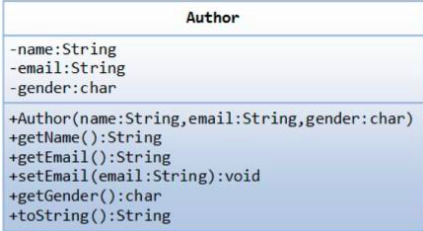
\includegraphics{uml-task1}
\caption{Диаграмма класса Author}\label{fig:uml-task1}
\end{figure}
\item По UML диаграмме класса, представленной на рисунке \ref{fig:uml-task2}.
написать программу, которая состоит из двух классов. Один из них Ball
должен реализовывать сущность мяч, а другой с названием TestBall
тестировать работу созданного класса. Класс Ball должен содержать
реализацию методов, представленных на UML. Диаграмма на рисунке
описывает сущность Мяч написать программу. Класс Ball моделирует
движущийся мяч.
\begin{figure}[H]
\centering
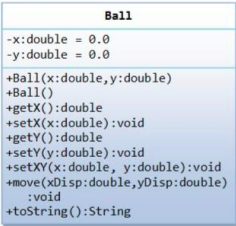
\includegraphics{uml-task2}
\caption{Диаграмма класса Ball}\label{fig:uml-task2}
\end{figure}
\item Создать класс точка Point, описывающий точку на плоскости.
Создать Circle класс, в котором одно поле представляет точку – центр
окружности, и добавить другие свойства, позволяющие задать точку на
плоскости. Создать третий класс Tester который использует для хранения
объектов массив объектов Circle и второе поле количество элементов в
массиве. 
\item Разработайте класс Shop для, реализуйте методы добавления и
удаления компьютеров в магазине, добавьте метод поиска в магазине
компьютера, нужного пользователю. Протестируйте работу созданных
классов. Данные для заполнения массива компьютеров вводятся с
клавиатуры пользователем. Для этого реализуйте интерфейс.
\item Разработайте и реализуйте класс Dog (Собака), поля класса
описывают кличку и возраст собаки. Необходимо выполнить следующие
действия: определить конструктор собаки, чтобы принять и
инициализировать данные экземпляра., включить стандартные методы
(аксессоры) для получения и установки для имени и возраста, включить
метод для перевода возраста собаки в “человеческий” возраст (возраст семь
раз собаки), включите метод ToString, который возвращает описание 
экземпляра собаки в виде строки. Создание класса тестера под названием
ПитомникСобак, реализует массив собак и основной метод этого класса
позволяет добавить в него несколько объектов собаки.
\item Создать класс, описывающий модель окружности (Circle). В
классе должны быть описаны нужные свойства окружности и методы для
получения и изменения этих свойств. Добавить методы для расчета
площади круга и длины окружности, а также метод позволяющий
сравнивать две окружности. При помощи класса CircleTest, содержащего
статический метод main(String[] args), протестировать работу класcа Circle. 
\item Создать класс, описывающий книгу (Book). В классе должны
быть описаны нужные свойства книги (автор, название, год написания и т.
д.) и методы для получения, изменения этих свойств. Протестировать
работу класса в классе BookTest, содержащим метод статический
main(String[] args). Создать класс книжная полка, в котором поля данных
класса это массив объектов типа книги (Book, и количество книг на
книжной полке. Написать методы класса, которые возвращают книги с
самым поздним и самым ранним сроком издания. Написать метод класса,
позволяющий расставить книги на книжной полке в порядке возрастания
года выпуска. Используйте реализацию отношений композиция классов
\item Напишите программу, которая меняет местами элементы
одномерного массива из String в обратном порядке. Не используйте
дополнительный массив для хранения результатов. 
\item Напишите программу Poker.java, которая должна имитировать
раздачу карт для игры в покер. Программа получает число n, задаваемое с
консоли пользователем, и раздает карты на n игроков (по 5 карт каждому)
из перетасованной колоды. Разделяйте пять карт, выданных каждому
игроку, пустой строкой.
\item Напишите программу HowMany.java, которая определит,
сколько слов Вы ввели с консоли.
\end{enumerate}
\section*{Программный код}
\begin{code}
\captionof{listing}{Класс Author}
\begin{Verbatim}[frame=single, fontsize=\footnotesize]
public class Author {
    private String name;
    private String email;
    private char gender;

    public Author(String name, String email, char gender){
        this.email = email;
        this.gender = gender;
        this.name = name;
    }

    public String getName() { return name; }
    public String getEmail() { return email; }
    public void setEmail(String email) { this.email = email; }
    public void setName(String name) {this.name = name; }
    public char getGender() { return gender; }

    @Override
    public String toString() {
        return "Author\n" +
                "name: " + name +
                "\nemail: " + email +
                "\ngender: " + gender;
    }
}
\end{Verbatim}
\end{code}
\begin{code}
\captionof{listing}{Тестовый класс TestAuthor}
\begin{Verbatim}[frame=single, fontsize=\footnotesize]
import java.util.Scanner;

public class TestAuthor {
    public static void main(String[] args) {
        Scanner source = new Scanner(System.in);
        System.out.println("input name");
        String name = source.nextLine();
        System.out.println("input email");
        String email = source.nextLine();
        System.out.println("input gender");
        char gender = source.next().charAt(0);
        Author author = new Author(name, email, gender);
        System.out.println("toString test");
        System.out.println(author.toString());
        author.setEmail("setEmail@gmail.com");
        author.setName("setName");
        System.out.println("getName test: " + author.getName());
        System.out.println("getEmail test: " + author.getEmail());
        System.out.println("getGender test: " + author.getGender());
    }
}
\end{Verbatim}
\end{code}
\begin{code}
\captionof{listing}{Класс Ball}
\begin{Verbatim}[frame=single, fontsize=\footnotesize]
public class Ball {
    private double x = 0.0;
    private double y = 0.0;

    public Ball(double x, double y) {
        this.x = x;
        this.y = y;
    }
    public Ball() {
        x = 0.0;
        y = 0.0;
    }

    public double getX() { return x; }
    public double getY() { return y; }
    public void setX(double x) { this.x = x; }
    public void setY(double y) {this.y = y; }
    public void setXY(double x, double y) { this.x = x; this.y = y; }

    public void move(double xDisp, double yDisp) {
        this.x += xDisp;
        this.y += yDisp;
    }

    @Override
    public String toString() {
        return "ball position\n" +
                "x: " + x +
                "\ny: " + y;
    }
}
\end{Verbatim}
\end{code}
\begin{code}
\captionof{listing}{Тестовый класс TestBall}
\begin{Verbatim}[frame=single, fontsize=\footnotesize]
import java.util.Scanner;

public class TestBall {
    public static void main(String[] args) {
        Scanner source = new Scanner(System.in);
        System.out.println("input start x");
        double x = source.nextDouble();
        System.out.println("input start y");
        double y = source.nextDouble();
        Ball ball = new Ball(x, y);
        System.out.println("toString test");
        System.out.println(ball.toString());
        ball.setX(1.0);
        ball.setY(1.0);
        ball.setXY(2.0, 2.0);
        ball.move(3.0, 3.0);
        System.out.println("getX and getY test");
        System.out.println("x: " + ball.getX() + "\ny: " + ball.getY());
    }
}
\end{Verbatim}
\end{code}
\begin{code}
\captionof{listing}{Класс Point}
\begin{Verbatim}[frame=single, fontsize=\footnotesize]
public class Point {
    private double x = 0.0;
    private double y = 0.0;

    public Point(double x, double y) {
        this.x = x;
        this.y = y;
    }
    public Point() {
        x = 0.0;
        y = 0.0;
    }

    public void setXY(double x, double y) { this.x = x; this.y = y; }
    public double getX() { return x; }
    public double getY() { return y; }

    public String toString() {
        return "x: " + x +
                "\ny: " + y;
    }
}
\end{Verbatim}
\end{code}
\begin{code}
\captionof{listing}{Класс Circle}
\begin{Verbatim}[frame=single, fontsize=\footnotesize]
public class Circle {
    private Point c;

    public Circle(double x, double y) {
        c = new Point(x, y);
    }

    public void newPoint(double x, double y) {
        Point point = new Point(x, y);
    }
    public void setC(double x, double y) { c.setXY(x, y); }
}
\end{Verbatim}
\end{code}
\begin{code}
\captionof{listing}{Тестовый класс Tester}
\begin{Verbatim}[frame=single, fontsize=\footnotesize]
package ru.mirea.prac2.task3;

public class Tester {
    public static void main(String[] args) {
        Circle[] circles = new Circle[5];
        circles[0] = new Circle(1, 2);
        circles[1] = new Circle(2, 1);
        circles[2] = new Circle(3, 3);
        circles[3] = new Circle(6, 7);
        circles[4] = new Circle(9, 9);
        int length = circles.length;
    }
}
\end{Verbatim}
\end{code}
\begin{code}
\captionof{listing}{Класс Computer}
\begin{Verbatim}[frame=single, fontsize=\footnotesize]
public class Computer {

    public int index;
    private String CPU;
    private String GPU;
    private String RAM;

    private String SSD;

    public Computer(int index, String CPU, String GPU, String RAM, String SSD){
        this.index = index;
        this.CPU = CPU;
        this.GPU = GPU;
        this.RAM = RAM;
        this.SSD = SSD;
    }

}
\end{Verbatim}
\end{code}
\begin{code}
\captionof{listing}{Класс Shop}
\begin{Verbatim}[frame=single, fontsize=\footnotesize]
import java.util.ArrayList;

public class Shop{
    private static int i = 0;

    private String address;
    private String working_hours;
    public ArrayList<Computer> warehouse = new ArrayList<>();

    public Shop(String address, String working_hours){
        this.address = address;
        this.working_hours = working_hours;
    }

    public void addComputer(int index, String  CPU, String GPU, String RAM, String SSD){
        Computer a = new Computer(index, CPU, GPU, RAM, SSD);
        warehouse.add(i, a);
        i++;
    }

    public void deleteComputer(int index){
        for (int j = 0; j < warehouse.size(); j++) {
            if(warehouse.get(j).index == index){
                warehouse.remove(j);
                break;
            }
        }
        System.out.println("Computer has been deleted");
    }

    public void search(int index){
        for (int j = 0; j < warehouse.size(); j++)
            if(warehouse.get(j).index == index) {
                System.out.println("Computer available");
                return;
            }
        System.out.println("Computer is not available atm");
    }
}
\end{Verbatim}
\end{code}

\begin{code}
\captionof{listing}{Тестовый класс TestShop}
\begin{Verbatim}[frame=single, fontsize=\footnotesize]
import java.util.Scanner;

public class TestShop {
    public static void main(String[] args) {
        Scanner scanner = new Scanner(System.in);
        Shop shop = new Shop("damn street 4206669", "23:00 - 23:30");
        System.out.println("Enter the amount of computers ");
        int numberC = scanner.nextInt();
        int currentIndex;
        String currentCPU, currentGPU, currentRAM, currentSSD;
        for (int i = 0; i < numberC; i++) {
            System.out.println("Enter the ID");
            currentIndex = scanner.nextInt();
            scanner.nextLine();
            System.out.println("Enter the CPU");
            currentCPU = scanner.nextLine();
            System.out.println("Enter the GPU");
            currentGPU = scanner.nextLine();
            System.out.println("Enter the RAM");
            currentRAM = scanner.nextLine();
            System.out.println("Enter the SSD");
            currentSSD = scanner.nextLine();
            shop.warehouse.add(i, new Computer(currentIndex, currentCPU, currentGPU, currentRAM, currentSSD));
            if (i == numberC - 1) {
                System.out.println("Database updated");
            } else {
                System.out.println("\nNext computer\n");
            }
        }
        shop.search(2);
    }
}
\end{Verbatim}
\end{code}

\begin{code}
\captionof{listing}{Класс Dog}
\begin{Verbatim}[frame=single, fontsize=\footnotesize]
public class Dog {
    private String nickname;
    private int age;

    public Dog(String nickname, int age){
        this.nickname = nickname;
        this.age = age;
    }

    public String getNickname() {
        return nickname;
    }

    public void setNickname(String nickname) {
        this.nickname = nickname;
    }

    public int getAge() {
        return age;
    }

    public void setAge(int age) {
        this.age = age;
    }

    public int DageH(){
        return age * 7;
    }

    @Override
    public String toString() {
        return "Dog{" +
                "nickname='" + nickname + '\'' +
                ", age=" + age +
                '}';
    }
}
\end{Verbatim}
\end{code}
\begin{code}
\captionof{listing}{Тестовый класс TestDog}
\begin{Verbatim}[frame=single, fontsize=\footnotesize]
public class TestDog {
    public static void main(String[] args) {
        ArrayList<Dog> arr = new ArrayList<>();
        Scanner sc = new Scanner(System.in);
        int quantity = 0;
        System.out.println("Enter the amount of dogs");
        quantity = sc.nextInt();
        sc.nextLine();
        String currentNickname;
        int currentAge;
        for (int i = 0; i < quantity; i++) {
            System.out.println("Enter the dog's nickname");
            currentNickname = sc.nextLine();
            System.out.println("Enter the dog's age");
            currentAge = sc.nextInt();
            sc.nextLine();
            arr.add(i, new Dog(currentNickname, currentAge));
            if (i == quantity){System.out.println("all dogs in the kennel"); break; } else { System.out.println("\nNext dog in the kennel:\n"); }
        }
        System.out.println(arr.get(1));
    }

}
\end{Verbatim}
\end{code}

\begin{code}
\captionof{listing}{Класс Circle}
\begin{Verbatim}[frame=single, fontsize=\footnotesize]
public class Circle {
    private int r;

    private int i = 0;

    private Circle[] circle = new Circle[2];
    private final double PI = 3.14;

    public Circle(int r){
        this.r = r;
    }

    public void setR(int r) {
        this.r = r;
    }

    public int getR() {
        return r;
    }

    public double getLength(){
        return 2*PI*r;
    }

    public double getSquare(){
        return PI * Math.pow(r, 2);
    }

    public void setCircle(int i, int newValue){
        circle[i].r = newValue;
    }

    public void comparison(Circle circle){
        if (circle.r < this.r){ System.out.println("The circle with r = "+this.r+" larger"); }
        else if (circle.r == this.r) { System.out.println("The circles are equal"); }
        else if (circle.r > this.r) { System.out.println("The circle with r = "+circle.r+" larger"); }
    }


}
\end{Verbatim}
\end{code}
\begin{code}
\captionof{listing}{Тестовый класс TestCircle}
\begin{Verbatim}[frame=single, fontsize=\footnotesize]
import java.util.Scanner;

public class TestCircle {
    public static void main(String[] args) {
        Scanner sc = new Scanner(System.in);
        System.out.println("Enter the radius of the circle");
        int currentR = sc.nextInt();
        Circle circle1 = new Circle(currentR);
        System.out.println(circle1.getLength());
        System.out.println(circle1.getSquare());
        sc.nextLine();
        System.out.println("Enter the radius of the circle 2");
        currentR = sc.nextInt();
        Circle circle2 = new Circle(currentR);
        sc.nextLine();
        System.out.println("Enter the radius of the circle 3");
        currentR = sc.nextInt();
        Circle circle3 = new Circle(currentR);
        circle1.comparison(circle2);
        circle2.comparison(circle3);
    }
}
\end{Verbatim}
\end{code}

\begin{code}
\captionof{listing}{Класс Book}
\begin{Verbatim}[frame=single, fontsize=\footnotesize]
public class Book {
    private String author;
    private String name;
    private int year;

    public Book(String author, String name, int year){
        this.author = author;
        this.name = name;
        this.year = year;
    }

    public String getAuthor() {
        return author;
    }

    public String getName() {
        return name;
    }

    public int getYear() {
        return year;
    }

    public void setAuthor(String author) {
        this.author = author;
    }

    public void setName(String name) {
        this.name = name;
    }

    public void setYear(int year) {
        this.year = year;
    }

}
\end{Verbatim}
\end{code}
\begin{code}
\captionof{listing}{Класс Bookshelf}
\begin{Verbatim}[frame=single, fontsize=\footnotesize]
public class Bookshelf {
    private Book[] warehouse;

    public Bookshelf(int n) {
        this.warehouse = new Book[n];
    }

    public Bookshelf() {
        this.warehouse = new Book[0];
    }

    public void setWarehouse(Book warehouse[]) {
        this.warehouse = warehouse;
    }


    public void print(){
        for (int i = 0; i < warehouse.length; i++) {
            System.out.println("Author: "+warehouse[i].getAuthor());
            System.out.println("Name: "+warehouse[i].getName());
            System.out.println("Year: "+warehouse[i].getYear());

        }
    }

    public void minYear(){
        int minYear = warehouse[0].getYear();
        for (int i = 0; i < 3; i++) {
            if(warehouse[i].getYear() < minYear){
                minYear = warehouse[i].getYear();
            }
        }
        System.out.println("Min year: "+minYear);
    }

    public void maxYear(){
        int maxYear = warehouse[0].getYear();
        for (int i = 0; i < 3; i++) {
            if(warehouse[i].getYear() > maxYear){
                maxYear = warehouse[i].getYear();
            }

        }
        System.out.println("Max year: "+maxYear);
    }

    public void sort_by_year(){
        for (int i = warehouse.length - 1; i > 0; i--) {
            for (int j = 0; j < i; j++) {
                if( warehouse[j].getYear() < warehouse[j + 1].getYear() ) {
                    Book tmp = warehouse[j];
                    warehouse[j] = warehouse[j + 1];
                    warehouse[j + 1] = tmp;
                }
            }
        }
    }
}
\end{Verbatim}
\end{code}
\begin{code}
\captionof{listing}{Тестовый класс TestBook}
\begin{Verbatim}[frame=single, fontsize=\footnotesize]
public class TestBook {
    public static void main(String[] args) {
        Scanner sc = new Scanner(System.in);
        Book[] warehouse = new Book[3];
        Bookshelf obj1 = new Bookshelf(3);
        String currentName;
        String currentAuthor;
        int currentYear;
        for (int i = 0; i < warehouse.length; i++) {
            System.out.println("enter " + (i + 1) + " author");
            currentAuthor = sc.nextLine();
            System.out.println("enter " + (i + 1) + " name");
            currentName = sc.nextLine();
            System.out.println("enter " + (i + 1) + " year");
            currentYear = sc.nextInt();
            warehouse[i] = new Book(currentAuthor, currentName, currentYear);
            sc.nextLine();
        }
        obj1.setWarehouse(warehouse);
        obj1.sort_by_year();
        obj1.print();
        obj1.maxYear();
        obj1.minYear();
    }
}
\end{Verbatim}
\end{code}

\begin{code}
\captionof{listing}{Класс Sort}
\begin{Verbatim}[frame=single, fontsize=\footnotesize]
public class Sort {
    public static void main(String[] args) {
        String[] a = new String[]{"1", "2", "3", "4", "5"};
        System.out.print("Before sorting:\t");
        for (int i = 0; i < a.length; i++) {
            System.out.print(a[i]+"\t");
        }
        String temp;
        for (int i = 0; i < a.length/2; i++) {
            temp = a[i];
            a[i] = a[a.length-i-1];
            a[a.length-i-1] = temp;
        }
        System.out.println();
        System.out.print("After sorting:\t");
        for (int i = 0; i < a.length; i++) {
            System.out.print(a[i]+"\t");

        }
    }
}
\end{Verbatim}
\end{code}

\begin{code}
\captionof{listing}{Класс Poker}
\begin{Verbatim}[frame=single, fontsize=\footnotesize]
import java.util.Scanner;

public class Poker {
    public static void main(String[] args) {
        int n;
        Scanner sc = new Scanner(System.in);
        System.out.println("Enter the number of players");
        n = sc.nextInt();
        String[] cards = { "2", "3", "4", "5", "6", "7", "8", "9", "10", "J", "Q", "K", "A"};

        String[] cardtype = { "Hearts", "Spades", "Diamonds", "Clubs"};

        int quantity = cards.length * cardtype.length;

        if ( n < 2){ System.out.println("Not enough people to play");}
        else if (n * 5 > quantity) { System.out.println("There are too many players");}

        String[] pack = new String[quantity];
        for (int i = 0; i < cards.length; i++) {
            for (int j = 0; j < cardtype.length; j++) {
                pack[cardtype.length * i + j] = cards[i] + " " + cardtype[j];
                System.out.println(pack[cardtype.length * i + j]);
            }

        }

        for (int i = 0; i < quantity; i++) {
            int k = i + (int) (Math.random() * (quantity-i));
            String temp = pack[k];
            pack[k] = pack[i];
            pack[i] = temp;

        }
        System.out.println();
        for (int i = 0; i < n * 5; i++) {
            System.out.println(pack[i]);
            if (i % 5 == 5 - 1){
                System.out.println();
            }
        }
    }
}
\end{Verbatim}
\end{code}

\begin{code}
\captionof{listing}{Класс HowMany}
\begin{Verbatim}[frame=single, fontsize=\footnotesize]
public class HowMany {
    public static void main(String[] args) {
        System.out.println("enter some text");
        Scanner sc = new Scanner(System.in);
        String string = sc.nextLine();
        StringTokenizer ins = new StringTokenizer(string);
        int cnt = 0;
        while (ins.hasMoreTokens()){
            cnt++;
            ins.nextToken();
        }
        System.out.println("amount of words in ur text: " + cnt);

    }
}
\end{Verbatim}
\end{code}
\section*{Вывод программы}
\begin{code}
\captionof{listing}{Вывод задания 1}
\begin{Verbatim}[frame=single, fontsize=\footnotesize]
input name
ivanov
input email
ivanov@mail.ru
input gender
m
toString test
Author
name: ivanov
email: ivanov@mail.ru
gender: m
getName test: setName
getEmail test: setEmail@gmail.com
getGender test: m
\end{Verbatim}
\end{code}
\begin{code}
\captionof{listing}{Вывод задания 2}
\begin{Verbatim}[frame=single, fontsize=\footnotesize]
input start x
0
input start y
1
toString test
ball position
x: 0.0
y: 1.0
getX and getY test
x: 5.0
y: 5.0
\end{Verbatim}
\end{code}
\begin{code}
\captionof{listing}{Вывод задания 4}
\begin{Verbatim}[frame=single, fontsize=\footnotesize]
Enter the amount of computers 
3
Enter the ID
1234
Enter the CPU
i7
Enter the GPU
1050Ti
Enter the RAM
4Gb
Enter the SSD
Sasung

Next computer

Enter the ID
543
Enter the CPU
i5
Enter the GPU
RTX2080
Enter the RAM
16Gb
Enter the SSD
Sasung

Next computer

Enter the ID
785
Enter the CPU
i3
Enter the GPU
MX150
Enter the RAM
2Gb
Enter the SSD
ADATA
Database updated
Computer is not available atm
\end{Verbatim}
\end{code}
\begin{code}
\captionof{listing}{Вывод задания 5}
\begin{Verbatim}[frame=single, fontsize=\footnotesize]
Enter the amount of dogs
2
Enter the dog's nickname
Rookie
Enter the dog's age
5

Next dog in the kennel:

Enter the dog's nickname
Sanya
Enter the dog's age
3

Next dog in the kennel:

Dog{nickname='Sanya', age=3}
\end{Verbatim}
\end{code}
\begin{code}
\captionof{listing}{Вывод задания 6}
\begin{Verbatim}[frame=single, fontsize=\footnotesize]
Enter the radius of the circle
20
125.60000000000001
1256.0
Enter the radius of the circle 2
10
Enter the radius of the circle 3
5
The circle with r = 20 larger
The circle with r = 10 larger
\end{Verbatim}
\end{code}
\begin{code}
\captionof{listing}{Вывод задания 7}
\begin{Verbatim}[frame=single, fontsize=\footnotesize]
enter 1 author
Amogus
enter 1 name
Sussus
enter 1 year
1984
enter 2 author
Bugaev
enter 2 name
Aleksander
enter 2 year
2022
enter 3 author
Ivanov
enter 3 name
Ivano
enter 3 year
2000
Author: Bugaev
Name: Aleksander
Year: 2022
Author: Ivanov
Name: Ivano
Year: 2000
Author: Amogus
Name: Sussus
Year: 1984
Max year: 2022
Min year: 1984
\end{Verbatim}
\end{code}
\begin{code}
\captionof{listing}{Вывод задания 8}
\begin{Verbatim}[frame=single, fontsize=\footnotesize]
Before sorting:	1	2	3	4	5	
After sorting:	5	4	3	2	1
\end{Verbatim}
\end{code}
\begin{code}
\captionof{listing}{Вывод задания 9}
\begin{Verbatim}[frame=single, fontsize=\footnotesize]
Enter the number of players
5
2 Hearts
2 Spades
2 Diamonds
2 Clubs
3 Hearts
3 Spades
3 Diamonds
3 Clubs
4 Hearts
4 Spades
4 Diamonds
4 Clubs
5 Hearts
5 Spades
5 Diamonds
5 Clubs
6 Hearts
6 Spades
6 Diamonds
6 Clubs
7 Hearts
7 Spades
7 Diamonds
7 Clubs
8 Hearts
8 Spades
8 Diamonds
8 Clubs
9 Hearts
9 Spades
9 Diamonds
9 Clubs
10 Hearts
10 Spades
10 Diamonds
10 Clubs
J Hearts
J Spades
J Diamonds
J Clubs
Q Hearts
Q Spades
Q Diamonds
Q Clubs
K Hearts
K Spades
K Diamonds
K Clubs
A Hearts
A Spades
A Diamonds
A Clubs

3 Hearts
K Diamonds
8 Hearts
4 Diamonds
A Spades

4 Spades
K Spades
A Hearts
2 Diamonds
8 Spades

Q Diamonds
7 Hearts
J Spades
A Diamonds
K Clubs

9 Spades
2 Clubs
10 Clubs
6 Clubs
4 Clubs

4 Hearts
6 Diamonds
9 Clubs
10 Spades
10 Hearts
\end{Verbatim}
\end{code}
\begin{code}
\captionof{listing}{Вывод задания 10}
\begin{Verbatim}[frame=single, fontsize=\footnotesize]
enter some text
wafeo fwaf wfe
amount of words in ur text: 3
\end{Verbatim}
\end{code}
\section*{Вывод}
В ходе данной лабораторной работы были изучены основные концепции объектно-ориентированного программирования, изучено понятие класса.
\end{document}